\chapter{Hasil Eksperimen di Rooftop Gedung 10 Unpar}
\label{lamp:C}

\section{Topologi Star}

\subsection{SensorA}
\begin{figure}[H] 
	\centering  
	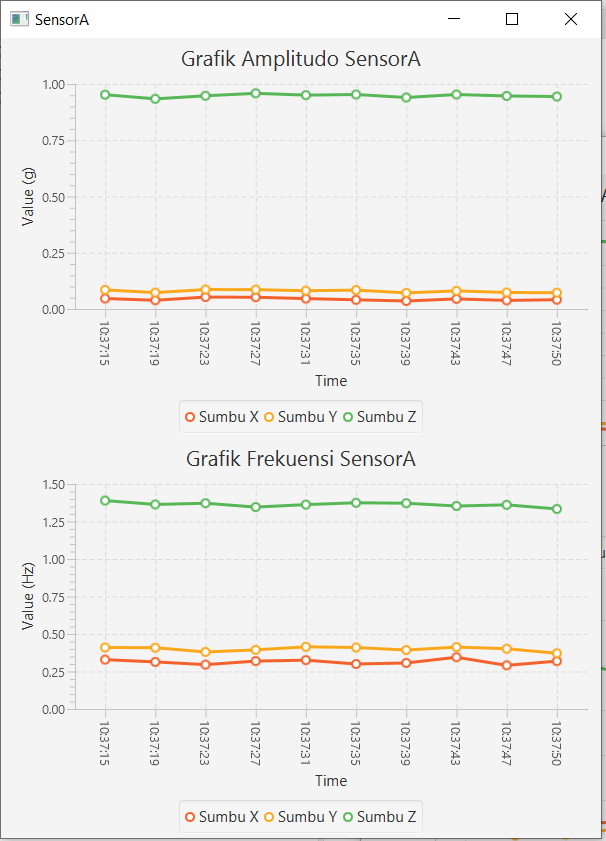
\includegraphics[scale=1]{Lampiran/HasilPengujian/sensorA_starRooftop2.PNG} 
	\caption[Grafik Monitoring getaran SensorA dengan topologi star]{Grafik Monitoring getaran SensorA dengan topologi star}
	\label{fig:grafik_A_star_rooftop} 
\end{figure}

\subsection{SensorB}
\begin{figure}[H] 
	\centering  
	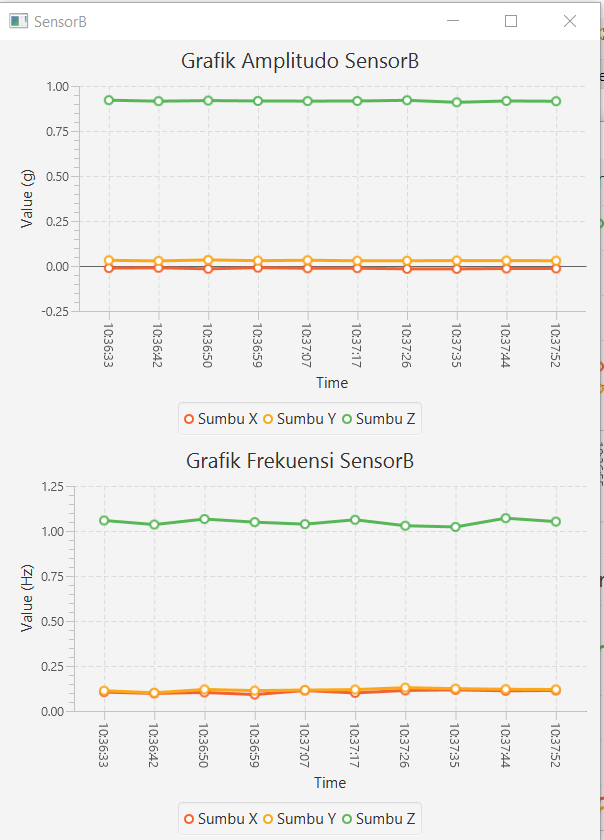
\includegraphics[scale=1]{Lampiran/HasilPengujian/sensorB_starRooftop2.PNG} 
	\caption[Grafik Monitoring getaran SensorB dengan topologi star]{Grafik Monitoring getaran SensorB dengan topologi star}
	\label{fig:grafik_B_star_rooftop} 
\end{figure}

\subsection{SensorC}
\begin{figure}[H] 
	\centering  
	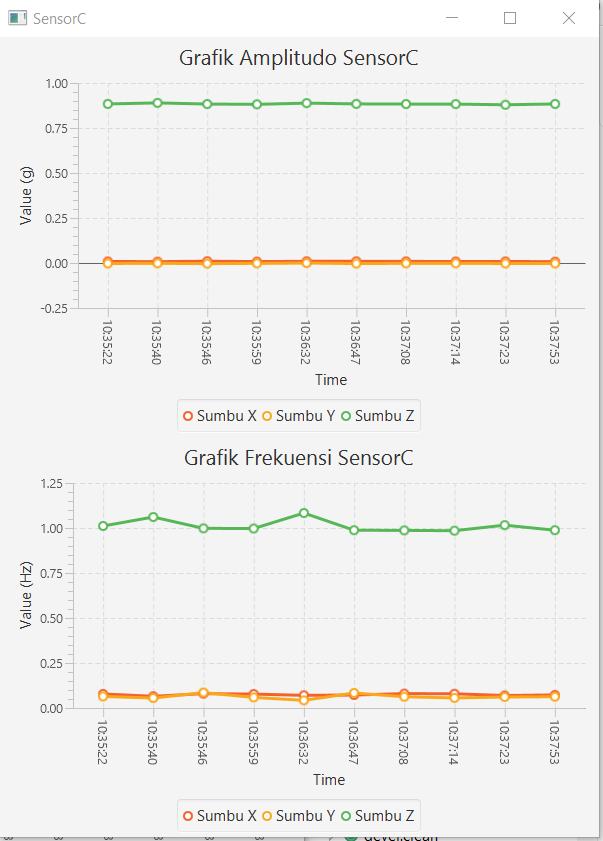
\includegraphics[scale=1]{Lampiran/HasilPengujian/sensorC_starRooftop2.PNG} 
	\caption[Grafik Monitoring getaran SensorC dengan topologi star]{Grafik Monitoring getaran SensorC dengan topologi star}
	\label{fig:grafik_C_star_rooftop} 
\end{figure}

\subsection{SensorD}
\begin{figure}[H] 
	\centering  
	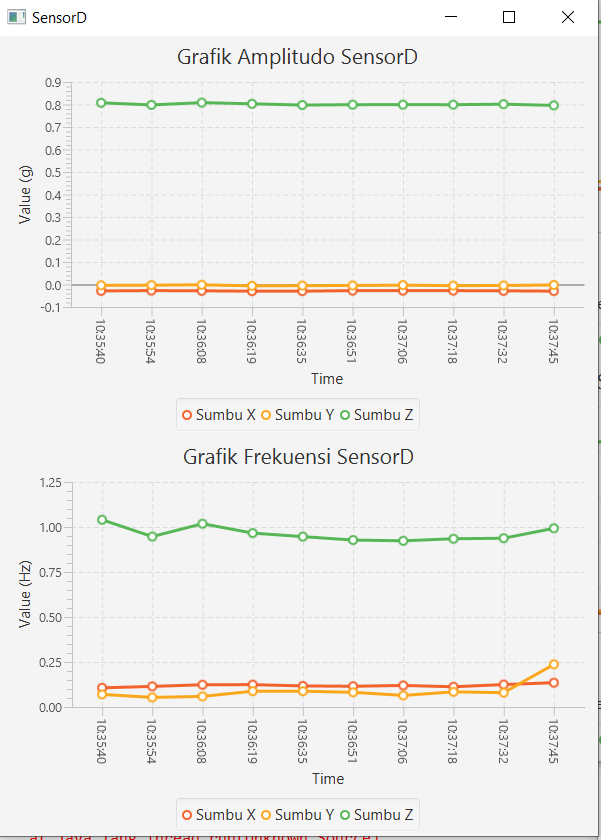
\includegraphics[scale=1]{Lampiran/HasilPengujian/sensorD_starRooftop2.PNG} 
	\caption[Grafik Monitoring getaran SensorD dengan topologi star]{Grafik Monitoring getaran SensorD dengan topologi star}
	\label{fig:grafik_D_star_rooftop} 
\end{figure}

\subsection{SensorE}
\begin{figure}[H] 
	\centering  
	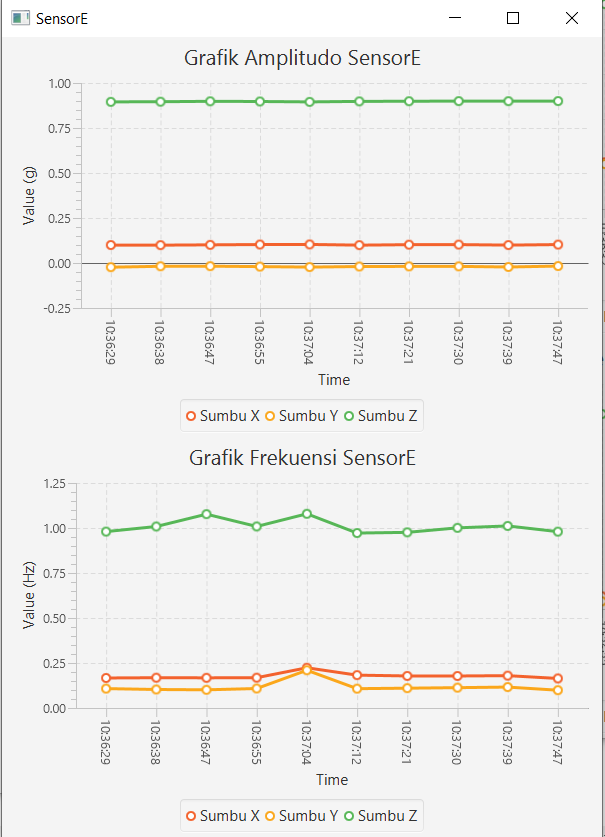
\includegraphics[scale=1]{Lampiran/HasilPengujian/sensorE_starRooftop2.PNG} 
	\caption[Grafik Monitoring getaran SensorE dengan topologi star]{Grafik Monitoring getaran SensorE dengan topologi star}
	\label{fig:grafik_E_star_rooftop} 
\end{figure}

\section{Topologi Tree}

\subsection{SensorA}
\begin{figure}[H] 
	\centering  
	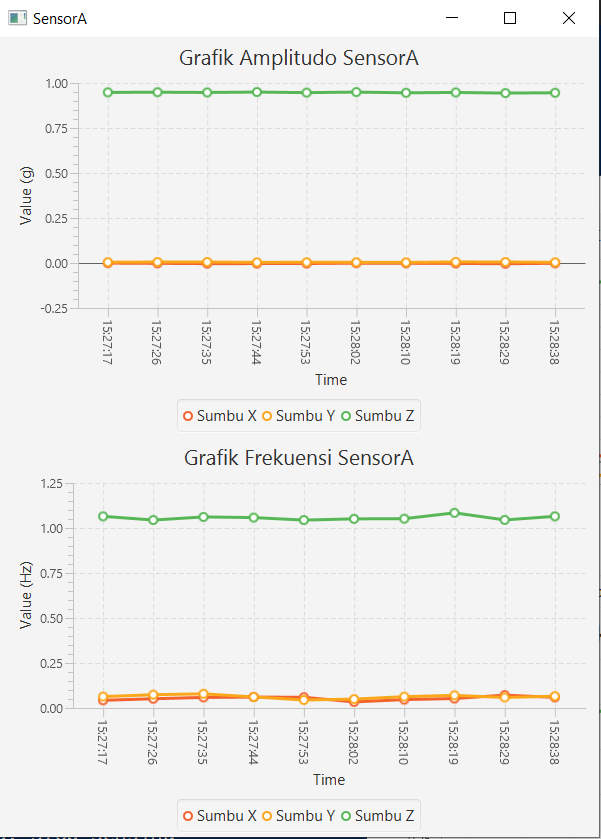
\includegraphics[scale=1]{Lampiran/HasilPengujian/sensorA_treeRooftop.PNG} 
	\caption[Grafik Monitoring getaran SensorA dengan topologi tree]{Grafik Monitoring getaran SensorA dengan topologi tree}
	\label{fig:grafik_A_tree_rooftop} 
\end{figure}

\subsection{SensorB}
\begin{figure}[H] 
	\centering  
	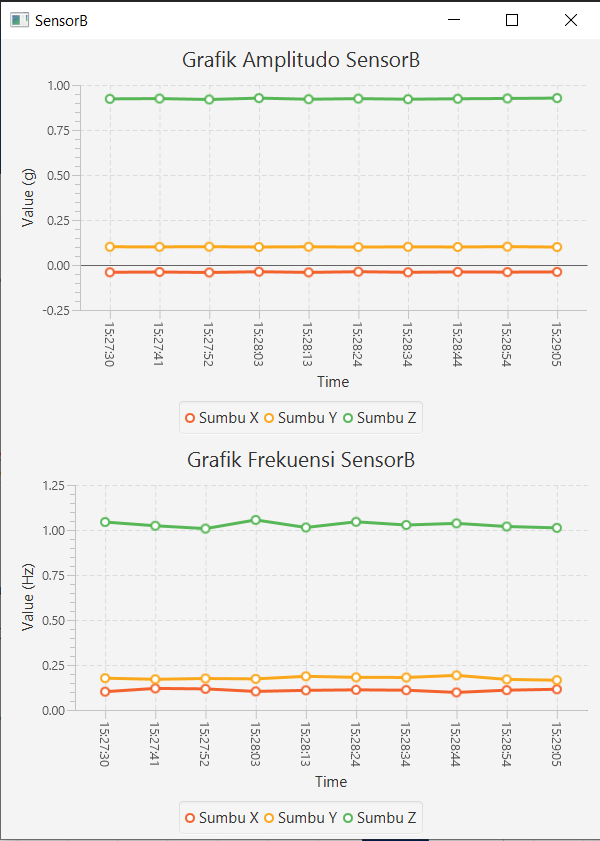
\includegraphics[scale=1]{Lampiran/HasilPengujian/sensorB_treeRooftop.PNG} 
	\caption[Grafik Monitoring getaran SensorB dengan topologi tree]{Grafik Monitoring getaran SensorB dengan topologi tree}
	\label{fig:grafik_B_tree_rooftop} 
\end{figure}

\subsection{SensorC}
\begin{figure}[H] 
	\centering  
	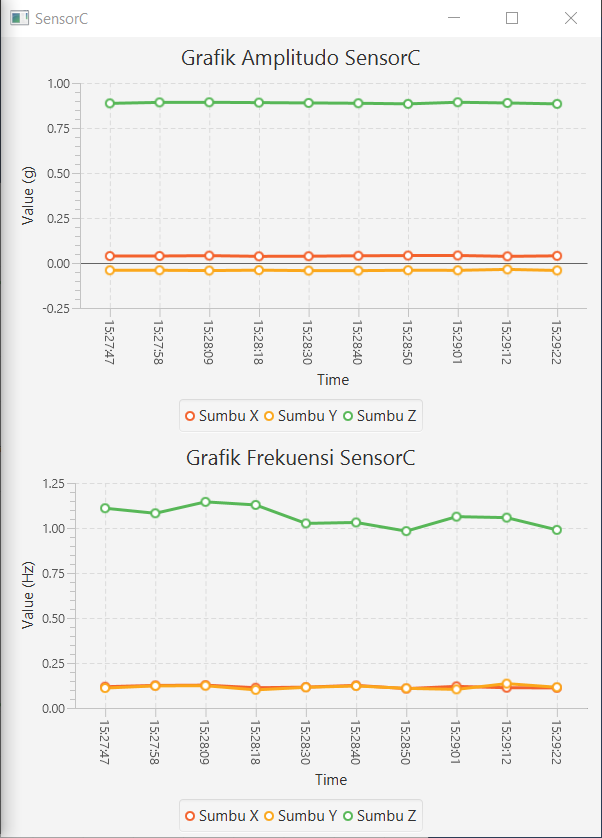
\includegraphics[scale=1]{Lampiran/HasilPengujian/sensorC_treeRooftop.PNG} 
	\caption[Grafik Monitoring getaran SensorC dengan topologi tree]{Grafik Monitoring getaran SensorC dengan topologi tree}
	\label{fig:grafik_C_tree_rooftop} 
\end{figure}

\subsection{SensorD}
\begin{figure}[H] 
	\centering  
	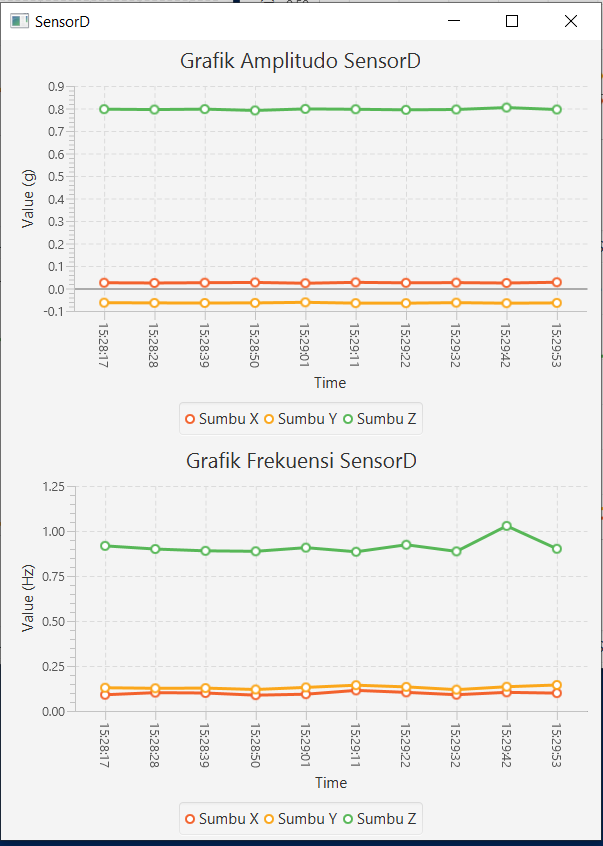
\includegraphics[scale=1]{Lampiran/HasilPengujian/sensorD_treeRooftop.PNG} 
	\caption[Grafik Monitoring getaran SensorD dengan topologi tree]{Grafik Monitoring getaran SensorD dengan topologi tree}
	\label{fig:grafik_D_tree_rooftop} 
\end{figure}

\subsection{SensorE}
\begin{figure}[H] 
	\centering  
	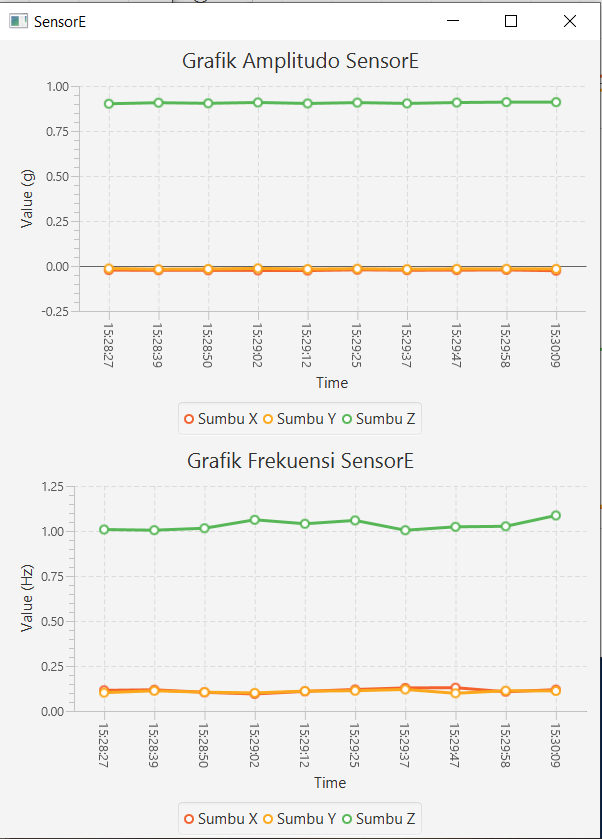
\includegraphics[scale=1]{Lampiran/HasilPengujian/sensorE_treeRooftop.PNG} 
	\caption[Grafik Monitoring getaran SensorE dengan topologi tree]{Grafik Monitoring getaran SensorE dengan topologi tree}
	\label{fig:grafik_E_tree_rooftop} 
\end{figure}